%
% Modelo de trabalho acadêmico (Teses, Dissertações, TCC)
% Documento principal
%
% Centro Federal de Educação Tecnológica de Minas Gerais - CEFET-MG
% Autor: Cristiano Fraga G. Nunes <cfgnunes@gmail.com>
%
% Projeto hospedado em: https://github.com/cfgnunes/latex-cefet-mg
%
%
% Informações:
%   Codificação utilizada: UTF-8
%   Tamanho da tabulação: 4 (espaços)


\documentclass[oneside]{abntex2-cefetmg}            % Imprimir apenas frente
%\documentclass[doubleside]{abntex2-cefetmg}        % Imprimir frente e verso

% Importações de pacotes
\usepackage[portuguese, onelanguage, lined, boxed, commentsnumbered, algoruled]{algorithm2e}                % Escrever algoritmos
\usepackage[alf, abnt-emphasize=bf, bibjustif, recuo=0cm, abnt-etal-cite=2, abnt-etal-list=0]{abntex2cite}  % Citações padrão ABNT
\usepackage[utf8]{inputenc}                         % Acentuação direta
\usepackage[T1]{fontenc}                            % Codificação da fonte em 8 bits
\usepackage{graphicx}                               % Inserir figuras
\usepackage{amsfonts, amssymb, amsmath}             % Fonte e símbolos matemáticos
\usepackage{booktabs}                               % Comandos para tabelas
\usepackage{verbatim}                               % Texto é interpretado como escrito no documento
\usepackage{multirow, array}                        % Múltiplas linhas e colunas em tabelas
\usepackage{indentfirst}                            % Endenta o primeiro parágrafo de cada seção.
\usepackage{microtype}                              % Para melhorias de justificação?
\usepackage{float}                                  % Utilizado para criação de floats
\usepackage{icomma}                                 % Uso de vírgulas em expressões matemáticas
%\usepackage{palatino}                               % Usa a fonte Palatino
\usepackage{times}                                 % Usa a fonte Times
%\usepackage{lmodern}                               % Usa a fonte Latin Modern
%\usepackage{color, colortbl}                       % Comandos de cores
%\usepackage{listings}                              % Importação de códigos fonte
%\usepackage[bottom]{footmisc}                      % Mantém as notas de rodapé sempre na mesma posição
%\usepackage{subfig}                                % Posicionamento de figuras
%\usepackage{scalefnt}                              % Permite redimensionar tamanho da fonte
%\usepackage{lscape}                                % Permite páginas em modo "paisagem"
%\usepackage{picinpar}                              % Dispor imagens em parágrafos
\usepackage[final]{pdfpages}

% Inclui o preâmbulo do documento
%
% Documento: Preâmbulo
%

\titulo{Em Direção a uma Métrica de Qualidade e Manutenibilidade de Código CSS}
%\title{Title in English}
%\subtitulo{}
\autor{Victor Carneiro Salvador}
\local{Belo Horizonte}
\data{Novembro de 2015}
\instituicao{Centro Federal de Educação Tecnológica de Minas Gerais}
\departamento{Departamento de Computação}
\programa{Curso de Engenharia de Computação}
\tipotrabalho{Trabalho Monográfico de Conclusão de Curso}
%\preambulo{Não será compilado.}
\orientador{Flávio Roberto dos Santos Coutinho}
%\orientador[Orientadora:]{Nome da orientadora}
\titulacaoOrientador{Prof. }
\instOrientador{Centro Federal de Educação Tecnológica de Minas Gerais -- CEFET-MG}
%\coorientador{Nome do coorientador}
%\coorientador[Coorientadora:]{Nome da coorientadora}
%\titulacaoCoorientador{Prof. Dr. }
%\instCoorientador{Centro Federal de Educação Tecnológica de Minas Gerais -- CEFET-MG}
\areaconcentracao{Engenharia de \textit{Software}}
\linhapesquisa{Qualidade de Código}


% Define as cores dos links e informações do PDF
\makeatletter
\hypersetup{
    portuguese,
    colorlinks,
    linkcolor=black,
    citecolor=black,
    filecolor=black,
    urlcolor=black,
    breaklinks=true,
    pdftitle={\@title},
    pdfauthor={\@author},
    pdfsubject={\imprimirpreambulo},
    pdfkeywords={}
}
\makeatother

% Redefinição de labels
\renewcommand{\algorithmautorefname}{Algoritmo}
\def\equationautorefname~#1\null{Equa\c c\~ao~(#1)\null}

% Cria o índice remissivo
\makeindex

% Início do documento
\begin{document}

    % Retira espaço extra obsoleto entre as frases
    \frenchspacing

    % Elementos pré textuais
    \pretextual
    %
% Documento: Capa
%

\makeatletter
\begin{capa}

    \hspace{-2.0cm}
    \begin{minipage}{0.19\textwidth}
        
\includegraphics[width=0.8\textwidth]{./04-figuras/cefet-logo}
    \end{minipage}
    \quad
    \hspace{-1.5cm}
    \begin{minipage}{.9\textwidth}
        \begin{center}
        \normalfont\scshape{\imprimirinstituicao}\\
        \normalfont\scshape{\imprimirdepartamento}\\
        \normalfont\scshape{\imprimirprograma}\\
        \abntex@ifnotempty{\imprimirareaconcentracao}
        {%
            \normalfont\scshape{\imprimirareaconcentracao}
        }
        \end{center}
    \end{minipage}

    \vspace*{200pt}

    \begin{center}
        \ABNTEXchapterfont\Large\scshape\imprimirtitulo
        \abntex@ifnotempty{\imprimirsubtitulo}{%
            {\ABNTEXchapterfont\Large\scshape: }{\ABNTEXchapterfont\large\scshape\imprimirsubtitulo}
        }
    \end{center}

    \vspace*{80pt}

    \begin{center}
        \large\normalfont\scshape\textbf\imprimirautor
    \end{center}

    \vspace*{10pt}

    \begin{center}
        \small\imprimirorientadorRotulo{} \imprimirTitulacaoOrientador \imprimirorientador \\
        \small\imprimirinstOrientador \\
        \abntex@ifnotempty{\imprimircoorientador}
        {%
            \begin{SingleSpacing}\par\end{SingleSpacing}
            \small\imprimircoorientadorRotulo{} \imprimirTitulacaoCoorientador \imprimircoorientador \\
            \small\imprimirinstCoorientador
        }
    \end{center}

    \vspace*{\fill}

    \begin{center}
        \normalfont\scshape{\imprimirlocal}\\
        \normalfont\scshape{\imprimirdata}
    \end{center}

\end{capa}
\makeatother
              % Capa
    %
% Documento: Folha de rosto
%

\makeatletter
\begin{folhaderosto}

    \begin{center}
        {\large\normalfont\scshape\textbf\imprimirautor}
    \end{center}

    \vspace*{150pt}

    \begin{center}
        \ABNTEXchapterfont\Large\scshape\imprimirtitulo
        \abntex@ifnotempty{\imprimirsubtitulo}{%
            {\ABNTEXchapterfont\Large\scshape: }{\ABNTEXchapterfont\large\scshape\imprimirsubtitulo}
        }
    \end{center}

    \vspace*{90pt}

    \abntex@ifnotempty{\imprimirpreambulo}{%
        \SingleSpacing
        \begin{tabular}{p{.24\textwidth}p{.15\textwidth}p{.44\textwidth}}
            & \multicolumn{2}{p{.6\textwidth}}{\small\hyphenpenalty=10000{\imprimirpreambulo}} \\ & & \\
            \abntex@ifnotempty{\imprimirareaconcentracao}
            {%
                & \multicolumn{2}{p{.6\textwidth}}{\small\hyphenpenalty=10000{\imprimirareaconcentracaoRotulo\imprimirareaconcentracao}} \\ & & \\
            }
            \abntex@ifnotempty{\imprimirlinhapesquisa}
            {%
                & \multicolumn{2}{p{.6\textwidth}}{\small\hyphenpenalty=10000{\imprimirlinhapesquisaRotulo\imprimirlinhapesquisa}} \\ & & \\
            }
            & \small\imprimirorientadorRotulo & \imprimirorientador \\
            & & \small\imprimirinstOrientador \\ & & \\
            \abntex@ifnotempty{\imprimircoorientador}
            {%
                & \small\imprimircoorientadorRotulo & \imprimircoorientador \\
                & & \small\imprimirinstCoorientador
            }
        \end{tabular}
    }

    \vspace*{\fill}

    \begin{center}
        \normalfont\scshape{\imprimirlocal}\\
        \normalfont\scshape{\imprimirdata}
    \end{center}

\end{folhaderosto}
\makeatother
       % Folha de rosto
    \makeatletter
\begin{folhadeaprovacao}
	\begin{center}
		\textbf{Centro Federal de Educação Tecnológica de Minas Gerais}\\~\\
		
		Curso de Engenharia de Computação \\~\\ 
		
		Avaliação do Trabalho de Conclusão de Curso
	\end{center}
	
	\hfill \break
	\hfill \break
	\noindent Aluno: \imprimirautor
	
	\noindent Título do Trabalho: \imprimirtitulo
	
	\noindent Data da defesa: 27/11/2015
	
	\noindent Horário: 14:00
	
	\noindent Local da defesa: Sala 101, Prédio 17 do CEFET-MG - Campus II
	\hfill \break
	\newline
	\begin{center}
	O  presente Trabalho de Conclusão de Curso foi avaliado pela seguinte banca:\\~\\ 
	Professor Flávio Roberto dos Santos Coutinho - Orientador \\
	Departamento de Computação \\
	Centro Federal de Educação Tecnológica de Minas Gerais \\~\\
	
	Professora Glívia Angélica Rodrigues Barbosa - Membro da banca de avaliação \\
	Departamento de Computação \\
	Centro Federal de Educação Tecnológica de Minas Gerais \\~\\
	
	Professor Ismael Santana Silva - Membro da banca de avaliação \\
	Departamento de Computação \\
	Centro Federal de Educação Tecnológica de Minas Gerais \\~\\
	\end{center}
\end{folhadeaprovacao}   % Folha de aprovação
    %%
% Documento: Dedicatória
%

\begin{dedicatoria}

Espaço reservado para dedicatória.
Inserir seu texto aqui...

\end{dedicatoria}
       % Dedicatória
    %%
% Documento: Agradecimentos
%

\begin{agradecimentos}

Inserir seu texto aqui...
(esta página é opcional)

\end{agradecimentos}
    % Agradecimentos
    %
% Documento: Epígrafe
%

\begin{epigrafe}

\textit{``O fator decisivo para vencer o maior obstáculo é, invariavelmente, ultrapassar o obstáculo anterior.'' (Henry Ford)}
(esta página é opcional)

\end{epigrafe}
          % Epígrafe
    %
% Documento: Resumo (Português)
%

\begin{resumo}

Escrever código CSS não é uma tarefa trivial, visto que algumas características da linguagem constantemente causam inconsistências arquiteturais que podem resultar em efeitos colaterais. Devido a essas características, podem ser identificados uma série de fatores que dificultam a construção, manutenção e evolução do código CSS. Estas etapas são essenciais durante o tempo de vida do \textit{software}, e isso não é diferente para aplicações \textit{web}. Sendo assim é necessário que seja encontrada uma forma de mitigar os possíveis impactos da modificação, ou evolução, do código CSS de um projeto \textit{web}. Uma forma de diminuir os impactos dessa etapa é criar uma métrica de qualidade que identifique o nível de manutenibilidade do código CSS. Essa necessidade ainda não foi suprida por nenhum trabalho acadêmico, portanto, é necessário ainda identificar quais são os aspectos que definem a qualidade do CSS. Para identificá-los, foi construído um questionário exploratório para fazer o levantamento das características do CSS que impactam na qualidade do código, visando uma forma de quantificar a manutenibilidade do código CSS. A partir da definição dos critérios de qualidade, foi construído um \textit{script} para o cálculo da métrica proposta, de forma a gerar dados para ela e o número de defeitos gerados a partir do código calculado. Através destes resultados é possível notar um progresso em direção à qualidade de código CSS. 

\textbf{Palavras-chave}: CSS. manutenibilidade. métrica. qualidade de código. Engenharia de Software. web.

\end{resumo}
         % Resumo na língua vernácula
    %%
% Documento: Resumo (Inglês)
%

\begin{resumo}[Abstract]

Translation of the abstract into english, possibly adapting or slightly changing the text in order to adjust it to the grammar of english educated.

\textbf{Keywords}: latex. abntex. template.

\end{resumo}
         % Resumo em língua estrangeira
    %
% Documento: Lista de figuras
%

\pdfbookmark[0]{\listfigurename}{lof}
\listoffigures*
\cleardoublepage
     % Lista de figuras
    %%
% Documento: Lista de tabelas
%

\pdfbookmark[0]{\listtablename}{lot}
\listoftables*
\cleardoublepage
     % Lista de tabelas
    %
% Documento: Lista de quadros
%

\pdfbookmark[0]{\listofquadrosname}{loq}
\listofquadros*
\cleardoublepage
     % Lista de quadros
    %%
% Documento: Lista de algoritmos
%

\newcommand{\algoritmoname}{Algoritmo}
\renewcommand{\listalgorithmcfname}{Lista de Algoritmos}

\floatname{algocf}{\algoritmoname}
\newlistof{listofalgoritmos}{loa}{\listalgoritmoname}
\newlistentry{algocf}{loa}{0}

\counterwithout{algocf}{chapter}
\renewcommand{\cftalgocfname}{\algoritmoname\space}
\renewcommand*{\cftalgocfaftersnum}{\hfill--\hfill}

\pdfbookmark[0]{\listalgorithmcfname}{loa}
\listofalgorithms
\cleardoublepage
  % Lista de algoritmos
    %
% Documento: Lista de abreviaturas e siglas
%

\begin{siglas}
    \item[CSS] \textit{Cascading Style Sheets}
    \item[DOM] \textit{Document Object Tree}    
    \item[HTML] \textit{Hypertext Markup Language}
    \item[W3C] \textit{Worl Wide Web Consortium}
    \item[WWW] \textit{World Wide Web}
\end{siglas}
      % Lista de abreviaturas e siglas
    %%
% Documento: Lista de símbolos
%

\begin{simbolos}
    \item[$ \Gamma $] Letra grega Gama
    \item[$ \lambda $] Comprimento de ondada
    \item[$ \in $] Pertence
\end{simbolos}
    % Lista de símbolos
    %
% Documento: Sumário
%

\pdfbookmark[0]{\contentsname}{toc}
\tableofcontents*
\cleardoublepage           % Sumário

    % Elementos textuais
    \textual
    %
% Documento: Introdução
%

\chapter{Introdução}\label{chap:introducao}
\label{chap:intro}

A \textit{world wide web}, originalmente proposta como um meio para compartilhamento de documentos por Tim Berners-Lee, torna-se cada vez mais popular, tendo passado a ser usada para a criação de páginas mais complexas e até mesmo de sistemas de informação, como comércio eletrônico, fóruns, clientes de email, portais de compartilhamento de vídeo etc.

Inicialmente proposto  por Håkon Wium Lie e Bert Bos, o \textit{Cascading Style Sheet} (CSS) propunha a separação do documento de conteúdo da apresentação das páginas \textit{web}. Sendo um dos três padrões fundamentais da W3C para desenvolvimento de conteúdo \textit{web}, juntamente com o HTML e o Javascript, o CSS se tornou largamente utilizado. Apesar das vantagens da separação estrutural, os códigos se tornaram complexos e de manutenibilidade onerosa \cite{Mesbah2012}. Escrever regras CSS não é uma tarefa trivial, as características da linguagem como herança e especificidade de seletores colocam os desenvolvedores constantemente em situações nas quais se questionam a efetividade das associações de propriedades escolhidas. Essas características podem prejudicar o que \citeonline{KellerNuss2010} definem como efetividade e eficiência de código CSS:

\begin{itemize}
	\item\textbf{Efetividade do código:} a folha de estilo é efetiva se o documento de conteúdo ao qual ele é aplicado renderiza da forma desejada.
	
	\item\textbf{Eficiência do código:} folhas de estilo que causam o mesmo efeito em um documento de conteúdo ainda pode diferir significativamente no modo em que ela aplica a associação de propriedade. Maximizar a eficiência do código CSS significa aplicar a associação de propriedades de uma forma que o esforço da autoria, manutenção e eventual reutilização seja minimizado.
\end{itemize}


\section{Justificativa}
Alguns cuidados têm de ser tomados ao se alterar um código CSS, muitas vezes propriedades podem sobrescrever outras, tornando parte do código inefetiva. Alterações de dimensão, ou alterações de visibilidade dos elementos podem causar defeitos na renderização de elementos vizinhos, parentes ou filhos. Estes efeitos colaterais são muito comuns em edição de páginas onde a definição de estilo está distribuída em vários arquivos.

Pode-se notar, então, a dificuldade de se manter um código CSS sem falhas durante a construção de uma página \textit{web}. Portanto, existe a necessidade de se manter um alto grau de manutenibilidade. A manutenibilidade de um sistema é definida como a facilidade com a qual um \textit{software}, ou componente, pode ser modificado para corrigir falhas, melhorar performance, ou adaptar-se à mudança de ambiente \cite{Ieee1990}. A partir desta definição, pode-se identificar uma medida de manutenibilidade para códigos CSS, considerando-se que onde houver alta complexidade haverá a necessidade de se manter o funcionamento, ou adaptação, da apresentação do documento.

As linguagens de folha de estilo, como o CSS, são muito pouco documentadas \cite{Marden1999,Geneves2012,Quint2007} e, como identificado por \citeonline{Mesbah2012}, analisar código CSS com uma perspectiva de manutenção ainda não foi explorada em nenhum trabalho científico. Portanto, há necessidade de se definir a qualidade do código CSS, com objetivo de se manter um nível de manutenibilidade da apresentação de páginas \textit{web}. Para medir este nível, será feita neste trabalho, uma proposta de métrica de qualidade de código CSS, focando a manutenção do código.

\section{Objetivos}
\label{sec:obj}

A manutenção e modificação de \textit{software} são etapas essenciais para o seu tempo de vida, e isso não é diferente para aplicações \textit{web}. Sendo uma tarefa essencial, e complexa, entende-se que seja necessário encontrar uma forma de mitigar os possíveis impactos na modificação, ou evolução, das folhas de estilo dos projetos \textit{web}.

Este trabalho tem por objetivo propor métricas de qualidade de código fonte relacionadas à manutenibilidade do código. Para tanto, será feito um levantamento das propriedades da linguagem que modificam a facilidade da manutenção de seu produto, considerando a visão do autor e os aspectos funcionais.             % Introdução
    %
% Documento: Fundamentação Teórica
%

\chapter{Fundamentação Teórica}
\label{chap:fund-teor}
\section{HTML}
\label{sec:html}
HTML é a linguagem principal para criação de documentos e aplicações na \textit{Web} para o uso de todos, em qualquer lugar \cite{W3Chtml2015}.

O documento HTML consiste em uma árvore de elementos e texto. Cada elemento é representado por uma \textit{tag} de abertura e uma de fechamento. As \textit{tags} têm de estar todas aninhadas completamente, sem haver sobreposição. Os elementos podem ter atributos que controlam o seu comportamento \cite{HTMLspec2014}. Na \autoref{fig:simpleHTML} está representada a estrutura básica de um documento HTML.

\begin{figure}[!htb]
	\centering
	\caption{Exemplo de arquivo HTML válido.}
	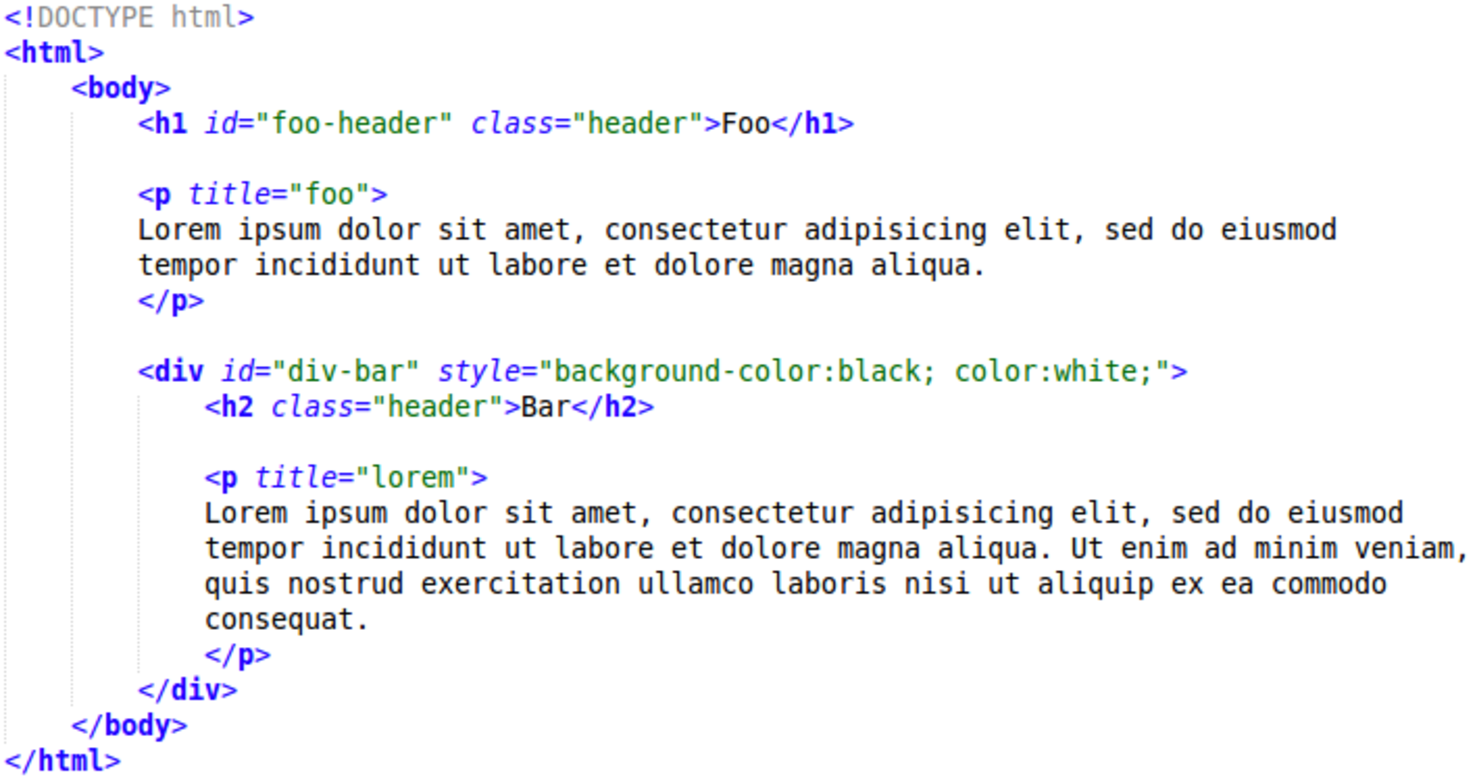
\includegraphics[width=1\textwidth]{./04-figuras/html_simples}
	\fonte{próprio autor}
	\label{fig:simpleHTML}
\end{figure}

\begin{figure}[!htb]
	\centering
	\caption{Estrutura de uma \textit{tag}.}
	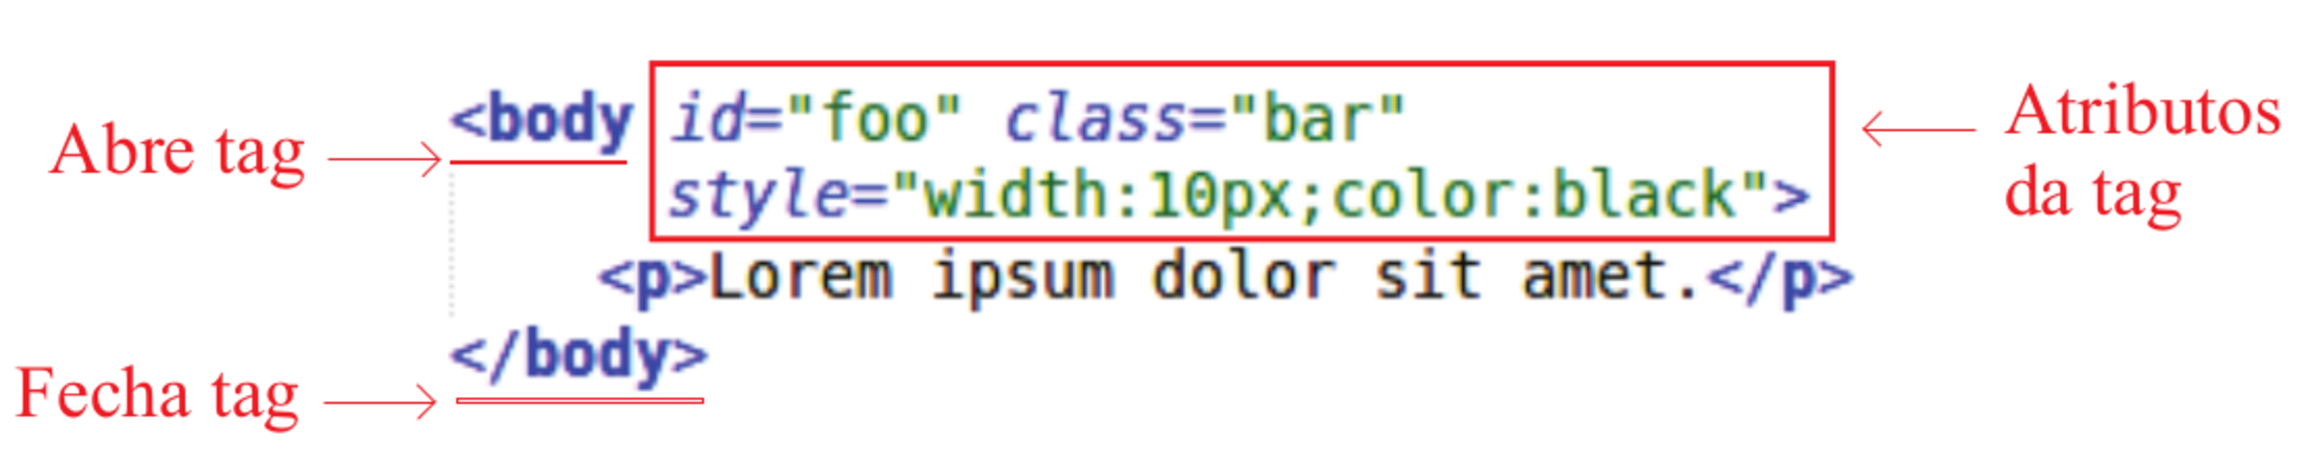
\includegraphics[width=.5\textwidth]{./04-figuras/tag_element_attr_marked}
	\fonte{próprio autor}
	\label{fig:tagStruct}
\end{figure}

Uma \textit{tag} HTML, pode possuir atributos que podem definir uma meta informação, com o objetivo de organizar o arquivo HTML, ou definir seu estilo. Esses atributos devem sempre ser definidos na \textit{tag} de abertura, e são representados por um par chave/valor. Podemos ver na \autoref{fig:tagStruct} uma estrutura simples de um \textit{tag} com os atributos \textit{id}, \textit{class} e \textit{style} definidos.

Pode-se notar na \autoref{fig:simpleHTML} a utilização dos atributos \textit{id}, \textit{title} e \textit{style}, que representam a identificação única do elemento, uma meta informação identificando a sua utilidade e o estilo aplicado a ele, respectivamente.

Dentro do documento HTML pode-se utilizar as \textit{tags} <style/> e <script/>, que definem escopos de estilo e linguagens de \textit{script}, como pode-se observar na \autoref{fig:styleScript}.

\begin{figure}[!htb]
	\centering
	\caption{Exemplo de arquivo HTML válido.}
	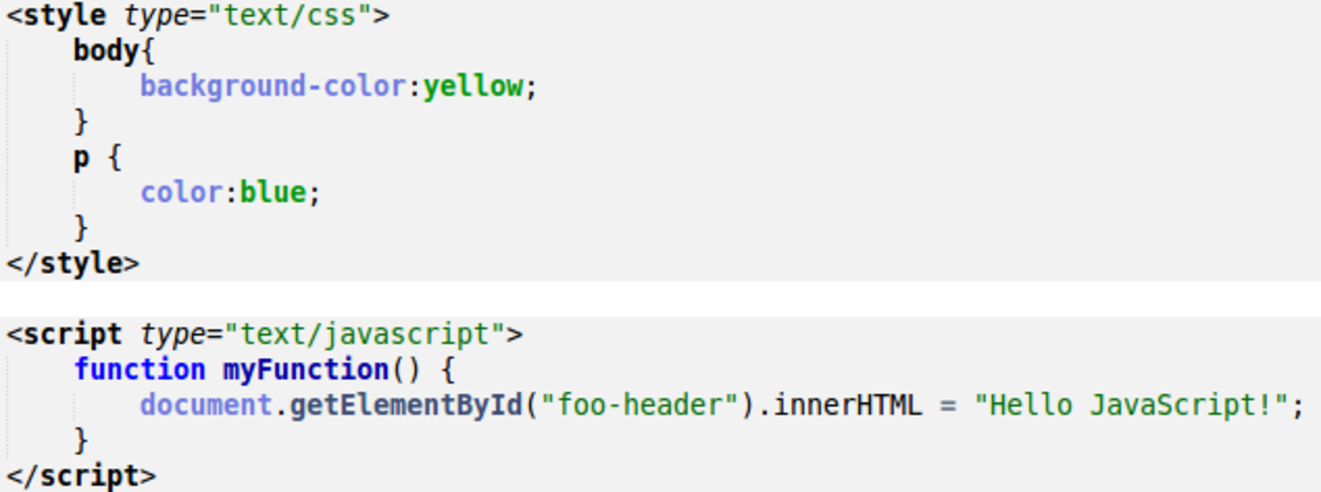
\includegraphics[width=1\textwidth]{./04-figuras/style_script}
	\fonte{próprio autor}
	\label{fig:styleScript}
\end{figure}

É uma boa prática de desenvolvimento \textit{web} manter as estruturas em arquivos diferentes, evitando ao máximo a utilização das \textit{tags} de escopo. Essa separação mantém uma organização do código, possibilita o reuso em outras páginas, ou até mesmo em outros sistemas, e também melhoram o desempenho, pois podem ser mantidos em cache, diminuindo a carga de dados necessária para renderização de um página \textit{web}. Porém, esta prática é difícil de gerenciar, dificultando a identificação de erros e o reuso de seus componentes.

Os navegadores \textit{web} (\textit{Browsers}) traduzem esse formato em uma árvore DOM (\textit{Document Object Model}). Uma árvore DOM é uma representação em memória de um documento, que possui vários nós, sendo que cada nó contém um elemento ou trecho de texto do documento.

\begin{figure}[!htb]
	\centering
	\caption{Exemplo de estrutura da árvore do DOM}
	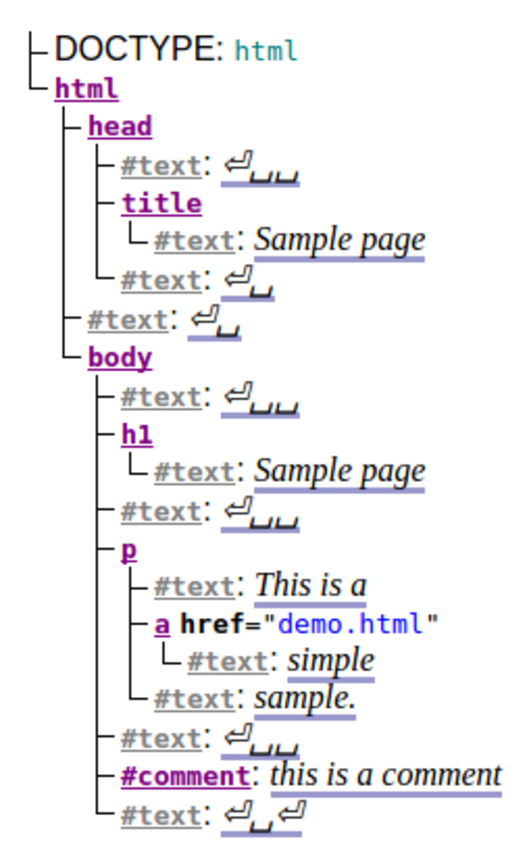
\includegraphics[width=0.3\textwidth]{./04-figuras/DOMsnippet}
	\fonte{\citeonline{HTMLspec2014}}
	\label{fig:domtree}
\end{figure}

Na \autoref{fig:domtree}, vê-se que o elemento raiz da árvore é o "html", que é sempre o primeiro elemento de um documento e que contém todos os outros. Cada elemento do HTML é representado por um nó, onde todos os nós que se encontram nos níveis abaixo deste são denominados descendentes (\textit{descendant}). Dentro da árvore DOM, os nós que se encontram exatamente um nível abaixo são os filhos (\textit{child}) e os nós que se encontram no mesmo nível são chamados de irmãos (\textit{sinbling}). Os nós denominados de \textit{text} são os que encapsulam os textos inseridos dentro dos elementos HTML, então estes serão os nós que existem em maior número no DOM.

A árvore DOM é utilizada para localização dos nós do HTML, as linguagens  CSS e javascript, utilizam da estrutura do DOM para encontrar os elementos e identificar quais são os elementos afetados por suas diretivas. O navegador determina a partir dos nós selecionados pelos seletores CSS, quais serão os elementos afetados pela regra.

\section{CSS}
\label{sec:CSS}
CSS é um mecanismo simples para adicionar estilo (\textit{e.g.}, fontes, cores, espaçamento) em documentos \textit{Web} \cite{W3Ccss2015}.

Uma folha de estilo \(C\) pode ser vista como um conjunto de regras \(R\), composto por regras simples \(R_i\), cada uma composta por um seletor \(S_i\) e um conjunto de pares: propriedade \(P_i\) e seus valores \(V_i\). Os seletores definem a quais elementos de um documento, serão aplicadas as propriedades definidas pela regra à qual elas pertencem \cite{Geneves2012}.

A \autoref{fig:cssExample} ilustra uma folha de estilo, com as regras representadas pelo conjunto de seletores, que precedem as chaves, e os pares "propriedade/valor" que as compões, dentro das chaves.

\begin{figure}[!htb]
	\centering
	\caption{Exemplo de uma folha de estilo $C$.}
	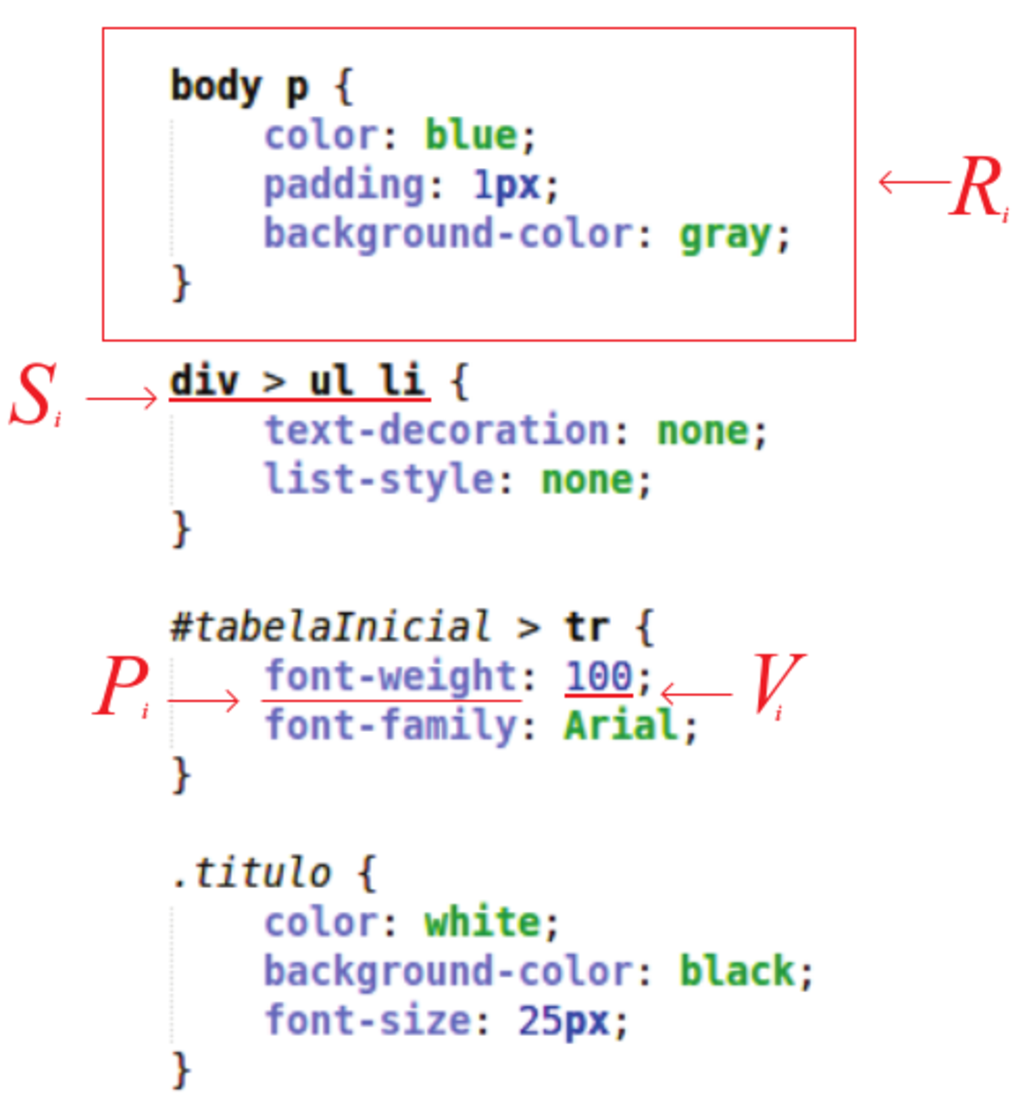
\includegraphics[width=0.3\textwidth]{./04-figuras/css_example_marked}
	\fonte{próprio autor}
	\label{fig:cssExample}
\end{figure}

\subsection{Seletores}
\label{subsec:seletores}
Um seletor é uma cadeia de uma, ou mais, sequências de seletores simples, separados por combinadores. Os seletores simples são cadeias de caracteres que representam um elemento do HTML: o seletor universal, representado pelo simbolo \(\ast\), indica que a regra será aplicada a todos os elementos que estejam no DOM. O seletor de elementos HTML é representado pelo nome da \textit{tag} de um elemento, por exemplo \(h1\). O seletor de classe, que seleciona todos os elementos que possuam o atributo \(class\) especificado pelo seletor, é utilizado escrevendo-se o nome da classe,  precedido de um ponto final (\(.\)). O seletor de \(id\), que seleciona o elemento do HTML que possua aquele \(id\), é utilizado escrevendo-se o identificador precedido pelo simbolo \(\#\). 
Simplificando, sem perder generalidade, pode-se considerar que regras são feitas de seletores únicos que definem uma única propriedade por vez. Os seletores \(S_i\), chamados de padrões na especificação do CSS \cite{CSSspec2009}, definem uma função booleana na forma:
\begin{equation}
	expression * element \rightarrow boolean
\end{equation}
que define se um elemento é, ou não, selecionado pela expressão do seletor.

Os combinadores são propriedades que definem relações entre os elementos de um documento. Existem três formas de combinadores: descendentes, filhos e irmãos. O combinador de descendente descreve qualquer elemento que esteja um nível abaixo na árvore DOM, e são representados pelo espaço em branco, \textit{e.g.} "$body\ p$". O combinador de filho descreve os elementos que estão exatamente um nível abaixo do nó, este combinador é representado pelo sinal de maior ($>$), \textit{e.g.} "$body > p$". O combinador de irmãos descreve os elementos que estão no mesmo nível da árvore, existem duas variações, uma para o próximo irmão adjacente ($+$) e um para todos os irmãos (\char`~).

Uma pseudo classe, é um elemento de seleção que especifica estado ou localização do elemento. Por exemplo, a pseudo classe ":nth-first-child(n)" identifica o n-ésimo elemento filho contando a partir do primeiro, podendo assim ser classificado como uma pseudo classe de localização. A pseudo classe ":hover" identifica um elemento que esteja sob o cursor do apontador (\textit{mouse}), sendo assim uma pseudo classe de estado. Ainda existem os seletores de atributos, que selecionam elementos que possuam determinados atributos, permitindo a utilização de expressões para seleções parciais, \textit{i.e.}, atributos que comecem, possuam ou terminem com uma cadeia de caracteres específicos.

Regras simples como as demonstradas na \autoref{fig:cssExample} são fáceis de se criar, mas quando utilizados combinadores e pseudo classes, a complexidade da autoria escala. Além da complexidade dos seletores, pode-se apontar o efeito cascata, gerado pelo mecanismo de precedência e aplicação das propriedades aos elementos HTML.

\subsection{Efeito Cascata}
\label{subsec:cascade}

O efeito cascata do CSS se dá devido à ordem de precedência dos valores de propriedades definidas para cada elemento. O mecanismo de renderização do navegador recebe uma lista desordenada dessas propriedades, e as organiza pela precedência das declarações delas. Essa ordem é definida de acordo com os critérios listados a seguir, em ordem decrescente de prioridade \cite{CSScascade2015}.

\begin{itemize}
	\item \textbf{Origem e Importância:} 
	Cada regra de estilo possui uma origem, que define onde ela estará na cascata, e a importância se refere à utilização, ou não, de um atributo que a explicita.
	\item \textbf{Escopo:}
	Uma declaração pode ter uma subárvore do DOM como escopo, afetando somente os elementos pertencentes a esta subárvore. Para declarações normais, o escopo mais interno tem prioridade, para as regras definidas como importantes as do escopo mais externo sobrescreverão.
	\item \textbf{Especificidade:}
	O calculo de especificidade conta a ocorrência de seletores de ID, classe e tipo (\textit{tags} e \textit{pseudo-elements}), e faz-se uma soma ponderada dessas ocorrências. A declaração com maior especificidade tem prioridade.
	\item \textbf{Ordem de aparição:}
	A última declaração no documento tem a maior prioridade. Isto significa que a localidade será levada em conta, para isso, considera-se que as folhas de estilo são concatenadas ao documento na ordem em que são declaradas.
\end{itemize}

Uma propriedade pode ter sua importância declarada explicitamente através do valor \textbf{!important}, que sobrescreverá todas as propriedades que possuírem maior prioridade. Se duas propriedades possuírem o valor \textbf{!important}, as outras especificações de prioridade terão efeito.

Outra propriedade do CSS que determina o funcionamento em cascata da aplicação de estilo é a herança. Cada propriedade de estilo possui um valor padrão de herança, que indica se aquela propriedade é propagada para seus filhos, essa herança pode ser definida explicitamente, a partir do valor da propriedade \textbf{inherit}. 

\section{Qualidade de \textit{Software}}

Com a finalidade de propor uma métrica, será necessário criar um arcabouço teórico sobre as técnicas e medições de qualidade de \textit{software} e código fonte.

A qualidade de \textit{software} faz um estudo sobre o produto do código fonte, considerando fatores produtivos e algumas vezes subjetivos. Em \citeonline{Pressman:2010}, destacam-se os fatores de qualidade de \textit{software}, definidos pela ISO 9126, apresentados a seguir:

\begin{itemize}
	\item \textbf{Funcionalidade}. Grau em que o \textit{software} satisfaz as necessidade declaradas.
	\item \textbf{Confiabilidade}. Período de tempo em que o \textit{software} está disponível para uso.
	\item \textbf{Usabilidade}. Grau em que o \textit{software} é fácil de usar.
	\item \textbf{Eficiência}. Grau em que o \textit{software} faz uso otimizado dos recursos do sistema.
	\item \textbf{Manutenibilidade}. Facilidade com a qual podem ser feitos reparos no \textit{software}.
	\item \textbf{Portabilidade}. Facilidade com a qual o \textit{software} pode ser transposto de um ambiente para outro.
\end{itemize}

Essas seis características chave apresentam a qualidade do produto de \textit{software}, que são difíceis de se medir quantitativamente e dependem da análise subjetiva de um especialista. Essa subjetividade torna as métricas difíceis de se reproduzir, portanto, é quase impossível determinar uma relação entre estados diferentes do produto.

\citeonline{Whitmire:1997} define a qualidade de \textit{software} orientado à objetos (OO) a partir de nove características distintas e mensuráveis de projetos OO:

\begin{itemize}
	\item \textbf{Tamanho}, definido em termos de quatro perspectivas: população, volume, comprimento e funcionalidade. População é medida pela contagem estática das entidades OO, tais como classes ou operações. Medidas de volume são medidas de população coletadas dinamicamente em função de um determinado instante de tempo. Comprimento é a medida de uma cadeia de elementos de projeto interconectadas, \textit{e.g}, a profundidade de uma árvore de herança. Métricas de funcionalidade fornecem uma indicação indireta do valor entregue ao cliente.
	\item \textbf{Complexidade} é determinada pela forma com a qual as classes OO de um projeto se inter-relacionam umas com as outras.
	\item \textbf{Acoplamento}, é definido pelas conexões físicas entre elementos de um projeto OO, \textit{e.g}, o número de colaborações entre as classes ou o número de mensagens passadas entre objetos.
	\item \textbf{Suficiência} é o grau das características exigidas de uma abstração ou o grau das características que um componente de projeto possui na sua abstração, do ponto de vista da aplicação corrente. Ou seja, um componente de \textit{software} é suficiente se reflete plenamente todas as propriedades do objeto de domínio de aplicação que representa.
	\item \textbf{Completeza} se diferencia de suficiência pelo conjunto de características com o qual se compara a abstração ou o componente de projeto. A completeza considera múltiplos pontos de vista da aplicação corrente. Como este critério considera diferentes pontos de vista, tem implicação direta no grau de reusabilidade da abstração.
	\item \textbf{Coesão} é determinada pelo grau em que o conjunto de propriedades que a abstração possui é parte do problema ou do domínio do projeto.
	\item \textbf{Primitividade} é o grau em que uma operação é atômica --- \textit{i.e.}, a operação não pode ser construída a partir de uma sequência de outras operações contidas na classe.
	\item \textbf{Similaridade} é o grau em que duas ou mais classes são semelhantes, em termos de sua estrutura, função ou finalidade.
	\item \textbf{Volatilidade} mede a probabilidade de que uma modificação venha a ocorrer em um componente de projeto OO.
\end{itemize}

Segundo \citeonline{Pressman:2010}, as métricas de qualidade de código-fonte também podem ser analisadas em nível de componente. Essas métricas são a de coesão, acoplamento e complexidade.

\subsection{Métricas de coesão}

\citeonline{Bieman1994} definem uma coleção de métricas que fornecem indicação da coesividade de um módulo. As métricas são definidas especificando cinco conceitos e medidas.

\begin{itemize}
	\item\textbf{Fatia de dados (\textit{data slice})} é um caminho retroativo ao longo de um módulo, que procura valores de dados que afetam a posição no módulo em que o caminho teve inicio.
	\item\textbf{Fichas de dados (\textit{data tokens})} são as variáveis especificadas para um módulo.
	\item\textbf{Fichas aglutinadas (\textit{glue tokens})} um conjunto de \textit{data tokens} que está contido em um, ou mais, \textit{data slices}.
	\item\textbf{Fichas superaglutinadas (\textit{superglue tokens})} são os \textit{data tokens} que estão contidos em todos os \textit{data slices}.
	\item A \textbf{aglutinação (\textit{stickiness})} relativa de uma ficha aglutinante é diretamente proporcional ao número de \textit{data slices} que ela aglutina.
\end{itemize}

As métricas de coesão definidas por \citeonline{Bieman1994} são de três tipos, coesão funcional forte (\textit{strong functional cohesion} --- SFC), coesão funcional fraca (\textit{weak function cohesion} --- WFC) e adesividade (\textit{adhesiveness}). 
Todas essas métricas de coesão variam de 0 a 1. Têm valor 0 quando um procedimento tem mais de uma saída e não exibe nenhum dos atributos de coesão indicados por uma métrica particular. Quando não há \textit{superglue tokens}, nenhuma ficha é comum a todos os \textit{data slices}, tem coesão funcional forte igual a zero. Quando não existem \textit{data tokens} comuns a mais de um \textit{data slice}, e o procedimento possui mais de um \textit{data slice}, exibe coesão funcional fraca zero e adesividade zero.

\subsection{Métricas de acoplamento}

O acoplamento de módulos fornece a indicação da conectividade de um módulo a outros módulos, dados globais e ambiente exterior.
A métrica para acoplamento de módulos proposta por \citeonline{Dhama:1995} que engloba acoplamento de dados e de fluxo de controle, acoplamento global e acoplamento ambiental. As medidas necessária para calcular acoplamento de módulos são definidas em termos de cada um dos três tipos de acoplamento mencionados.
Para acoplamento de dados e de fluxo de controle,
\begin{description}
	\item$d_i$ = número de parâmetros de dados de entrada
	\item$c_i$ = número de parâmetros de controle de entrada
	\item$d_o$ = número de parâmetros de dados de saída
	\item$c_o$ = número de parâmetros de controle de saída
\end{description}
Para acoplamento global,
\begin{description}
	\item$g_d$ = número de variáveis globais usadas como dados
	\item$g_c$ = número de variáveis globais usadas como controle
\end{description}
Para acoplamento ambiental,
\begin{description}
	\item$w$ = número de módulos chamados (\textit{fan-out})
	\item$r$ = número de módulos que chamam o módulo sendo considerado (\textit{fan-in})
\end{description}

Usando essas medidas, pode-se indicar um acoplamento de módulo, $m_c$. À medida que o valor de $m_c$, aumenta, o acoplamento global do módulo diminui.

\subsection{Métricas de complexidade}

Diversas métricas de \textit{software} podem ser calculadas para determinar a complexidade do fluxo de controle do programa. Muitas delas são baseadas no diagrama de fluxo.
As métricas de qualidade podem ser usadas para prever informação crítica sobre confiabilidade e manutenibilidade de sistemas de \textit{software} a partir da análise automática do código-fonte, ou informação do projeto procedimental. Métricas de complexidade também fornecem realimentação durante o projeto de \textit{software} para ajudar a controlar a atividade de projeto \cite{Pressman:2010}. Fornecendo informações detalhadas sobre os módulos de \textit{software}, durante o teste e manutenção, ajudando a localizar áreas de potencial instabilidade.

A métrica de complexidade mais amplamente usada (e debatida) para \textit{software} de computador é a complexidade ciclomática, desenvolvida por \citeonline{McCabe:1989}.          % Fundamentação teórica
    %
% Documento: Trabalhos Relacionados
%

\chapter{Trabalhos Relacionados}

Existem poucos trabalhos que tratem de qualidade de código CSS na literatura, e como \citeonline{Mesbah2012} identificou, não existem trabalhos que analisem o código em função da manutenibilidade.

Trabalhos como o de \citeonline{KellerNuss2010}, que analisa a qualidade de código CSS em uma perspectiva de avaliar a diferença em códigos de autoria humana e os auto gerados. Enquanto \citeonline{Mesbah2012} propõe uma ferramenta para auxiliar na manutenção de código, considerando a definição de efetividade e eficiência \cite{KellerNuss2010}, afim de determinar regras inefetivas e removê-las do código.

\citeonline{KellerNuss2010} propõe uma medida de qualidade do código CSS baseando-se na abstração do seletor. Esse trabalho é baseado no argumento de que o objetivo do código CSS é a reutilização de suas regras, a abstração do seletor é então definida pela sua utilização no escopo geral do HTML, considerando que seletores com id são os menos abstratos possíveis. Este trabalho não conseguiu encontrar uma relação forte com a complexidade de código CSS e o nível de abstração, de forma que os autores a consideraram uma medida fraca, se utilizada de forma exclusiva, deixando em aberto a proposta de métricas que a corroborem, ou cooperem com ela na medida de qualidade do código CSS.

Em \citeonline{Quint2007} ferramentas de auxílio na autoria de CSS são avaliadas, e a forma de avaliação do código, como estrutura de dados e método de avaliação do código. O trabalho de \citeonline{Quint2007} apresenta uma proposta de ferramenta didática que auxiliará na criação de folhas de estilo, de uma forma a auxiliar o entendimento da aplicação das propriedades e regras. Em seu trabalho \citeonline{Quint2007} identifica fatores que tornam a tarefa de autoria de código CSS não trivial.

     % Trabalhos relacionados
    %
% Documento: Metodologia
%

\chapter{Metodologia}

O primeiro passo da execução do trabalho consistiu na conceituação de qualidade do código CSS. Esse objetivo foi alcançado por meio de referências bibliográficas e de uma pesquisa do tipo \textit{survey} aplicada a desenvolvedores que escrevem código CSS em seu dia a dia, com níveis de experiência variados. 

Essa abordagem foi escolhida pelo fato de não haver, na literatura, uma definição canônica do que é qualidade de código CSS. Para isso foi construído um questionário, com o intuito de identificar os parâmetros de qualidade a partir da experiência dos desenvolvedores.

A partir dos resultados do questionário, foram identificados os critérios de avaliação que impactam na manutenibilidade do código CSS. Com a análise e os resultados obtidos para os critérios, de acordo com as hipóteses levantadas pelo autor, foram determinados os pesos de cada critério, para a execução dos testes individuais das folhas de estilo. Nesta etapa, foi obtido um resultado numérico representando o cálculo dos pesos para os critérios encontrados no código CSS.

% Tem que recomeçar essa frase e explicar que automatizado foi o teste, a avaliação foi na unha, na raça e no sangue
A partir dos valores encontrados nos testes, foram identificadas as relações entre o índice proposto e a quantidade de falhas identificadas em sistemas \textit{web} de código aberto. Utilizando uma base de projetos de \textit{software} de código aberto, foi feita uma análise e a referência cruzada, entre o valor obtido pela métrica do código CSS e o número de problemas reportados no projeto relacionados a alterações em código CSS.

\section{Questionário}

A pesquisa \textit{survey} é uma forma de obtenção de dados ou informações sobre características, ações ou opiniões de um determinado conjunto de pessoas, indicado como representante de uma população-alvo, por meio de um instrumento de pesquisa, normalmente um questionário \cite{Freitas2000}. 

O interesse de uma pesquisa desse tipo é produzir descrições quantitativas de uma população. No caso deste trabalho, o objetivo é identificar, de forma quantitativa, as características identificadas pelos desenvolvedores como sendo as que classificam a qualidade do código CSS. Para tanto, foi aplicado um questionário exploratório, com o objetivo de identificar os conceitos do CSS considerados centrais para a associação de qualidade do código.

\section{Proposta da Métrica}

As métricas de qualidade de código são indicadores numéricos baseados em características das linguagens de programação. Para este trabalho, essas características foram definidas a partir dos resultados obtidos no questionário. A métrica de qualidade para código CSS aqui descrita, foi calculada a partir da presença e frequência de alguns dos recursos da linguagem, identificados pelos desenvolvedores no questionário, considerados impactantes para a manutenibilidade do código.

\section{Avaliação dos Resultados}

A partir da métrica proposta, foi desenvolvida uma ferramenta automática de cálculo da métrica. O programa lê um arquivo CSS, identifica as regras definidas e, a partir da definição proposta, calcula o valor obtido por este arquivo. Além do arquivo CSS, o arquivo HTML que o inclui também foi considerado para o cálculo.

Com os valores da métrica calculada, foi testada sua aderência a um projeto de código aberto, utilizando como indicador de manutenibilidade o número de defeitos cadastrado na ferramenta de controle de tarefas do mesmo. Utilizando de versões antigas, fez-se um histórico de modificação da métrica e o número de defeitos cadastrados, relacionados com CSS e o layout da página, com o objetivo de avaliar o comportamento do indicador de manutenibilidade com os resultados obtidos no projeto ao longo do tempo.           % Metodologia
    %
% Documento: Resultados Esperados
%

\chapter{Resultados Preliminares}

A partir de uma análise sobre qualidade de software, métricas de qualidade e fundamentos teóricos do funcionamento do CSS, construiu-se uma pesquisa exploratória, em forma de um questionário, para identificação dos aspectos mais relevantes no processo de manutenção de uma folha de estilo e das características do código fonte que estão relacionadas à sua qualidade.

\section{Construindo o questionário}
Elaborou-se o questionário com os seguintes objetivos:

\begin{itemize}
	\item Identificar os aspectos da linguagem que mais impactam na legibilidade;
	\item Identificar os parâmetros que definem qualidade de código no ponto de vista dos entrevistados;
	\item Identificar aspectos mais custosos para manutenção;	
\end{itemize}

A partir da coleta das respostas, pode-se analisar os pesos de cada aspecto de qualidade do código CSS em função da manutenibilidade do estilo. Identificando as maiores ocorrências de efeitos colaterais, definindo quais são as técnicas para manter legibilidade mais utilizadas e quais aspectos de organização do código são mais relevantes.

Viu-se necessária a avaliação da complexidade de alguns aspectos da linguagem, a partir do ponto de vista do profissional, então o questionário foi construído com uma seção onde é avaliado, com base em um trecho de código, a dificuldade de se dar manutenção, cada trecho foi elaborado de acordo com um aspecto da linguagem que possam causa algum tipo de complicação. Esses aspectos foram escolhidos de acordo com as ponderações do autor, com base nos estudos realizados.

A propriedade dificuldade, atribuída por cada pessoa a um determinado conjunto de regras e propriedades, é subjetiva e depende fortemente da experiência do individuo. Portanto construiu-se o questionário com perguntas visando a classificação do respondente de acordo com o seu nível de conhecimento, a partir dessa classificação será possível ponderar as respostas de acordo com o nível dos respondentes.            % Resultados
    %
% Documento: Conclusão
%

\chapter{Conclusão}

Muitas propriedades clássicas de qualidade de código, e até mesmo propriedade de qualidade como coesão e acoplamento, para linguagens orientadas a objeto, não se aplicam diretamente ao CSS. Mas isso não impede que seja traçada uma relação entre o CSS e essas propriedades.

Através do questionário, executado como piloto, notou-se alguns ajustes que devem ser feitos para coletar com eficiência os dados necessários para propormos uma métrica. Com o questionário publicado, espera-se conseguir um número mínimo de cinquenta respostas ao questionário, para que possa ser feita a analise das respostas e identificar as propriedades da linguagem.

\section{Próximos passos}

Após a coleta dos dados do questionário, será proposta a métrica, a partir de valores dos aspectos identificados com a análise dos dados. A análise dos dados será feita de levando-se em conta o nível de conhecimento dos respondentes, como uma ponderação da variância da subjetividade da impressão de dificuldade.

Será construído uma ferramenta de calculo automático da métrica, para o levantamento e execução dos testes de aderência com os projetos de código aberto avaliados. Para tal será feita a comparação da pontuação da métrica de uma folha de estilo, com o número de problemas identificados na página \textit{web} relacionado à ela, buscando essas páginas em um repositório de código aberto. Ao final do trabalho serão avaliados os resultados obtidos, para identificar a validade da métrica proposta.             % Conclusão

    % Elementos pós textuais
    \postextual
    %
% Documento: Referências Bibliográficas
%

\bibliography{./refbase}    % Geração automática das referências por meio do arquivo 'refbase.bib'
       % Referências
    %
% Documento: Apêndices
%

\begin{apendicesenv}
\partapendices

\chapter{Nome do Apêndice}
\label{chap:apendicex}

Inserir seu texto aqui...

\chapter{Nome do Apêndice}
\label{chap:apendicey}

Inserir seu texto aqui...

\end{apendicesenv}
         % Apêndices
    %%
% Documento: Anexos
%

\begin{anexosenv}
\partanexos

\chapter{Nome do Anexo}
\label{chap:anexox}

Inserir seu texto aqui...

\chapter{Nome do Anexo}
\label{chap:anexoy}

Inserir seu texto aqui...

\end{anexosenv}
            % Anexos
    %\printindex                                             % Índice remissivo

\end{document}
